\section{Instalación de la paquetería de java}
%%%%%%%%%%%%%% RESUMEN 5%%%%%%%%%%%%%%%%%%
Primeramente será necesario instalar el open-jdk de java en el sistema, esto con el objetivo de permitir la ejecución de los algoritmos de minería de datos que serán ejecutados por el map reduce haciendo uso de java. Para realizar esta tarea realizaremos lo siguiente:
Acceder a la terminal GNU con privilegios de root e ingresar el siguiente comando.

\begin{enumerate}
	\item
	\begin{lstlisting} 
	root@maestro:~# apt-get install openjdk-8-jdk openjdk-8-jre
 	\end{lstlisting}

\begin{figure}[!htbp]
	\hypertarget{fig:instalacionjava}{\hspace{1pt}}
	\begin{center}
		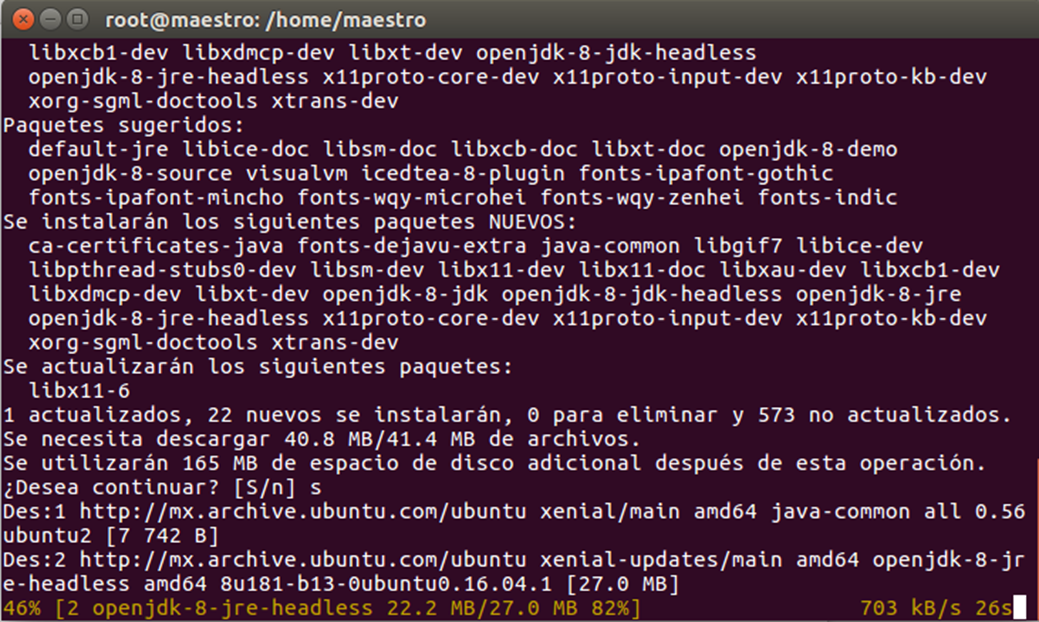
\includegraphics[width=.7\textwidth]{capitulo5/images/im1.png}
		\caption{Instalación de java en el nodo maestro}
		\label{fig:instalacionjava}
	\end{center}
\end{figure}

Este programa ocupara 165MB de espacio de disco y nos pedirá que confirmemos su instalación a lo que se contestará 
	\item ‘S’ 
para que proceda con la instalación.
Una vez que esta termine se podrá consultar la versión de java en el sistema con el comando

	\begin{lstlisting} 
	root@maestro:~# java -version
 	\end{lstlisting}
 	
\begin{figure}[!htbp]
	\hypertarget{fig:instalacionjava2}{\hspace{1pt}}
	\begin{center}
		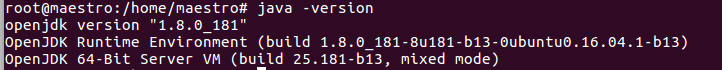
\includegraphics[width=.7\textwidth]{capitulo5/images/im2.png}
		\caption{Versión de java}
		\label{fig:instalacionjava2}
	\end{center}
\end{figure}
\end{enumerate}
%\subsubsection{Aspirante}
%\begin{itemize}
%	\item \textbf{Tarea 1. Administrar pagos realizados en sucursal}: Esta tarea permite al contador general mantener actualizado el status de pago de los aspirantes que realizaron la operación en sucursal bancaria, esto mediante las tareas : \textbf{Tarea 1.1. Generar Línea de captura}, \textbf{Tarea1.2. Actualizar pagos con la información de BANAMEX}, \textbf{Tarea1.3. Autorización de pagos}. Es importante mencionar que el actor solo podrá realizar dichas tareas cuando la convocatoria de ingreso tenga asociada toda la información correspondiente a las evaluaciones y haya cupos disponibles en la asignación de citas para la aplicación de las mismas, esto es, que la convocatoria no haya llegado a su límite de aspirantes a evaluar.
%	 \begin{itemize}
%	 	
%	
%	\item \textbf{Tarea 1.1. Generar Línea de captura}: Esta tarea le permite al actor, generar la línea de captura de un aspirante que la solicite de forma personal. Es importante mencionar que esta acción se logrará una vez que el aspirante haya aceptado los términos y condiciones de pagos desde su cuenta personal.
%	
%	
%	\item \textbf{Tarea1.2.	Actualizar pagos con la información de BANAMEX}: Esta tarea permite al actor, actualizar la información del status de pago de los aspirantes por medio de un archivo, el cual es proporcionado por BANAMEX. Es importante mencionar que el actor deberá de realizar los cambios pertinentes en el archivo para que este pueda ser interpretado por el sistema.
%		
%	\item \textbf{Tarea1.3. Autorización de pagos}: Esta tarea permite al actor establecer el estado de pago de un aspirante como exitoso, esto en el caso de que el aspirare haya realizado el pago y no se haya visto reflejado en el sistema por un problema externo. Cabe mencionar que esta tarea deberá de manejarse en casos muy específicos, ya que el sistema no registrará un monto al aspirante, simplemente le permitirá continuar con su proceso de admisión. 
%		 \end{itemize}
%\end{itemize}
%
%%A continuación se describen a detalle las funcionalidades del sistema, en función de que el aspirate pueda realizar cada una de las tareas descritas anteriormente. 
%
%
%
